\chapter{Título provisório do segundo capítulo}
É difícil ver o noticiário hoje sem se deparar com as Inteligências Artificiais (IAs).
Contudo, entre o uso de ChatGPT para trabalhos escolares, trabalhadores preocupados com perder o emprego para uma máquina, e até alguns com medo da humanidade ser inteiramente aniquilada num apocalipse da era digital, o uso de IAs é tão mais comum quanto mais dissimulado.

A culpa disso é do fato que ``Inteligência Artificial'' está muito mais próximo de uma expressão de marketing feita para atrair a atenção do que de um termo técnico.
Ela pressupõe uma semelhança entre o pensamento orgânico, tal como humanos o fazem, e um suposto pensamento sintético que, como há de ser visto nesse capítulo, é inteiramente dessemelhante a seu equivalente vivo.

Por trás da Inteligência Artificial há um conjunto de técnicas estatísticas e computacionais que fazem o chamado \textit{aprendizado de máquina} ou \textit{aprendizado estatístico}.
Antes de entender \textit{como} um computador pode aprender, é necessário responder \textit{por que} se quer que ele aprenda.
Há muito que um computador pode fazer sem a necessidade desse treinamento: isso inclui fazer contas, navegar pela Internet, assistir a um filme, tipografar uma monografia, entre outros.
Então, o que diferencia essas atividades de uma Inteligência Artificial?

A resposta é que essas atividades podem ser (e são) descritas por meio de código, o que requer representá-las como um conjunto de instruções claras e objetivas: uma receita de como as realizar.
É fácil elaborar uma receita de como reproduzir um vídeo, por exemplo.
O computador deverá localizar o arquivo que contém o vídeo, abri-lo, decodificá-lo e reproduzi-lo, convertendo as informações numéricas para cores a uma determinada taxa de vezes por segundo.
Por mais que cada passo aqui descrito possa ser desmembrado em tantos outros mais, qualquer programa de computador é descritível como um conjunto de instruções.
Todo processador é construído aos moldes de uma Arquitetura de Conjunto de Instruções (ISA, do inglês \textit{Instruction Set Architecture}), um modelo abstrato que delimita, simplificadamente, como se pode programá-lo.
Um dos componentes disso é um conjunto de instruções que o processador pode executar, para o qual \textit{todos} os programas que são usados devem ser reduzidos.
Essas instruções são coisas simples, como ``coloque tal valor em tal lugar'', ``some tal valor com tal valor'' e ``faça isso se tal valor for verdadeiro''.

É possível criar uma ``receita para escrever''?
Ou uma ``receita para recomendar vídeos''?
Isto é, um conjunto de instruções objetivas que permita realizar essas ações?
Não. 
E é aqui que entra o uso de uma IA: aproximar objetivamente processos que não podem ser descritos assim.

\section{Regressões Lineares}
Observe o seguinte gráfico com o valor da anomalia da temperatura média do globo terrestre em relação à média do século 20, entre 1970 e 2025:

\begin{figure}[H]
    \centering
    \caption{Gráfico da anomalia (°C) em função do tempo (anos), 1970-2025}
    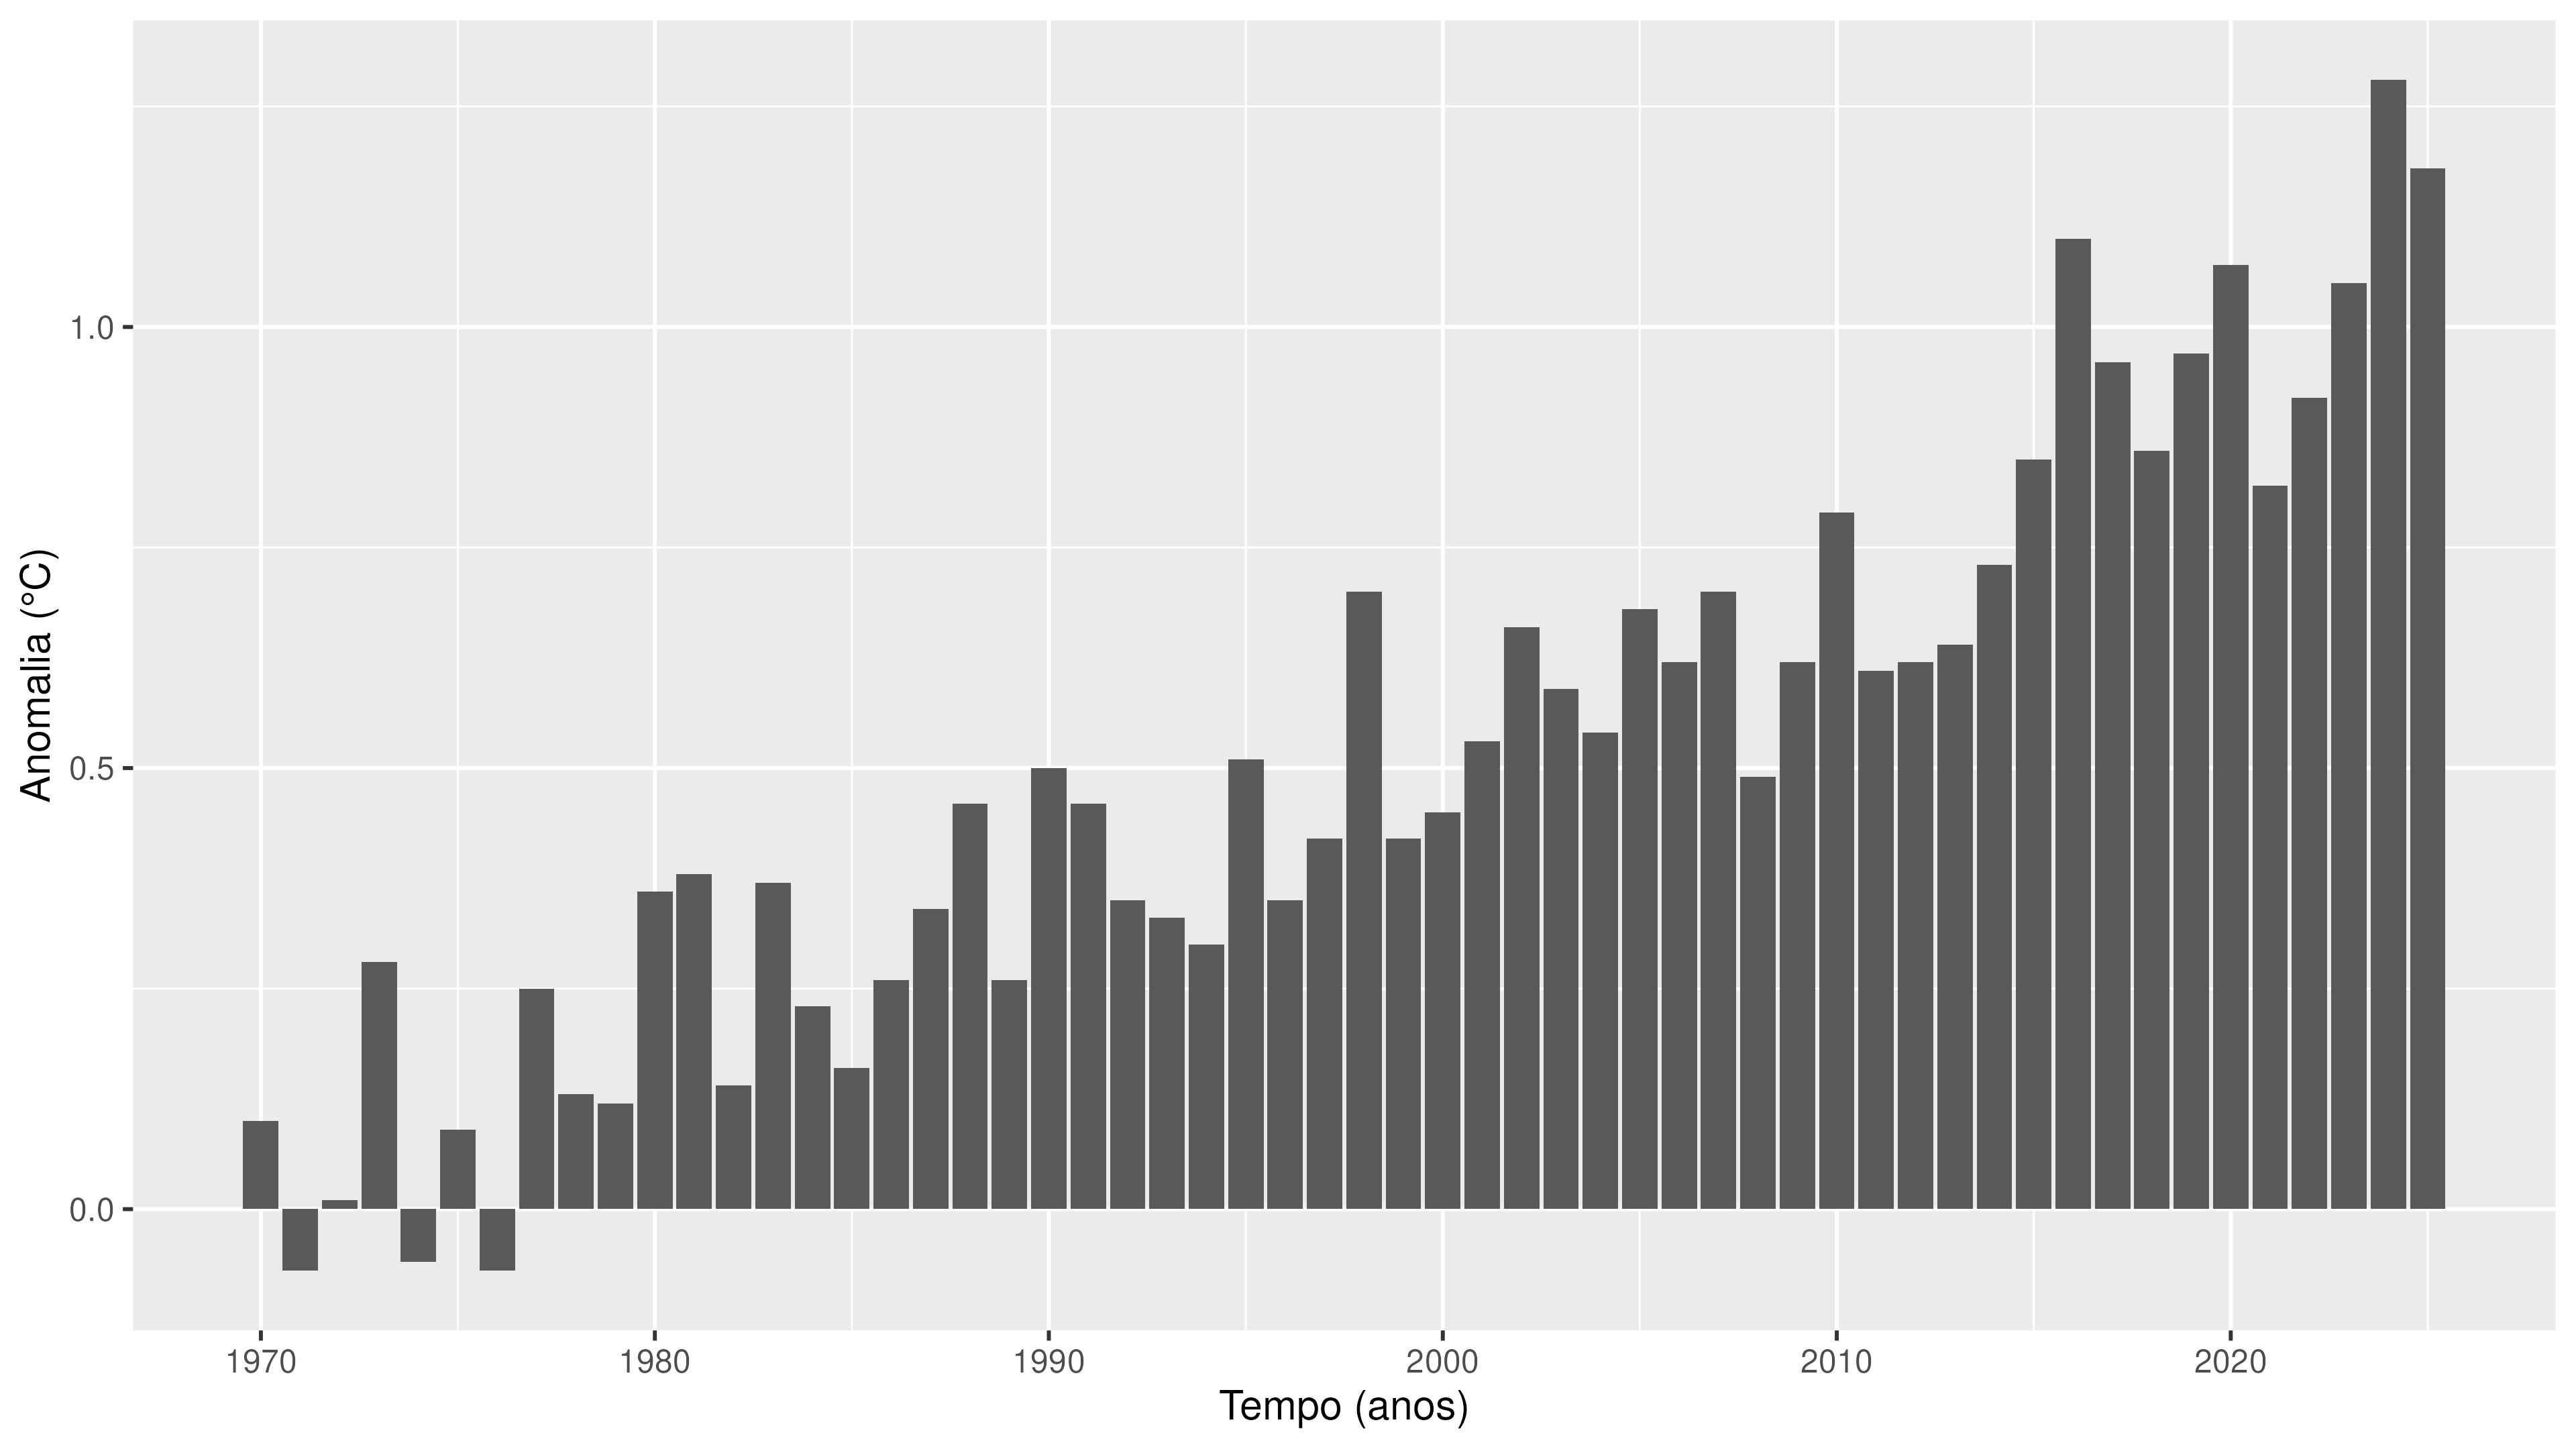
\includegraphics[width=\linewidth]{static/R/plot/anom-1-hist.png}
    \label{fig:2:anom-1-hist}
\end{figure}

Empiricamente, é possível perceber que existe uma tendência nesses dados, que seguem aproximadamente uma reta.
Porém, é difícil determinar precisamente de quanto é essa tendência, e para onde o gráfico continuará. 
Isso se deve ao fato de que o planeta Terra é um sistema complexo: ele não segue uma ordem do tipo ``aumente 0,5°C ao ano''.
Na metáfora da seção anterior, é impossível estabelecer uma receita para a temperatura do planeta em função do ano.

Pode-se, contudo, aproximá-la.
Sabe-se, a partir desses dados, como o modelo deve se comportar.
Não é possível, principalmente quando se trata de algo tão simples como uma reta, que ele abarque cada mínima mudança e inconsistência; é, afinal, uma aproximação.

Qual deverá ser a forma desse modelo?
Matematicamente, uma reta pode ser definida por meio de uma função linear, que, nesse caso, assumiria a forma de

\begin{equation}
A(t) = t\cdot\beta_1 + \beta_0
\end{equation}

Isto é, a anomalia $A$, em função do tempo $t$, pode ser definida como o tempo $t$ multiplicado por um coeficiente $\beta_1$ somado a um coeficiente estático $\beta_0$.
Assim, para determinar a anomalia, $t$ deve ser transformado, segundo os parâmetros $\beta_0$ e $\beta_1$ que, até agora, \textit{não se sabe quais são}.
Intuitivamente, $\beta_1$ é a inclinação da reta e $\beta_0$ a altura dela.
A grande pergunta, portanto, é quais são esses coeficientes, ou seja, como $t$ deve ser mudado para obter $A$.

Para determinar esses dois coeficientes, $\beta_0$ e $\beta_1$, é necessário primeiro conceber uma maneira de comparar dois modelos, e descobrir qual deles mais se aproxima do fenômeno aproximado.
Uma maneira muito simples de fazer isso é, para cada ano, contabilizar a distância entre o valor previsto pelo modelo e a observação real.
O objetivo da criação do modelo, assim, passa a ser reduzir ao máximo possível esse erro.
Comumente, ao invés de simplesmente usar o erro, é considerado o erro elevado ao quadrado; assim, erros menores são menos penalizados, e erros maiores serão ainda mais penalizados, pois seu valor crescerá com mais rapidez.
Essa abordagem é chamada de ``mínimos quadrados'', pois almeja minimizar os quadrados dos erros.

O processo de descobrir $\beta_0$ e $\beta_1$ é conhecido como \textit{aprendizado} ou \textit{treinamento}.
Ele envolve inicializar esses valores com um ``chute'', e, gradualmente, melhorá-los.
Para isso, muda-se ou $\beta_0$ ou $\beta_1$, incrementando-o por pouco. 
Se a mudança for bem-vinda, ou seja, diminuir o erro, ela é mantida; caso contrário, o original é melhor.
Ao repetir esse processo várias vezes, a reta será acomodada nos coeficientes com menor valor de erro.

No caso da figura \ref{fig:2:anom-1-hist}, isso se parece com 

\begin{figure}[H]
    \centering
    \caption{Gráfico da anomalia (°C) em função do tempo (anos), 1970-2025, com modelo de regressão linear}
    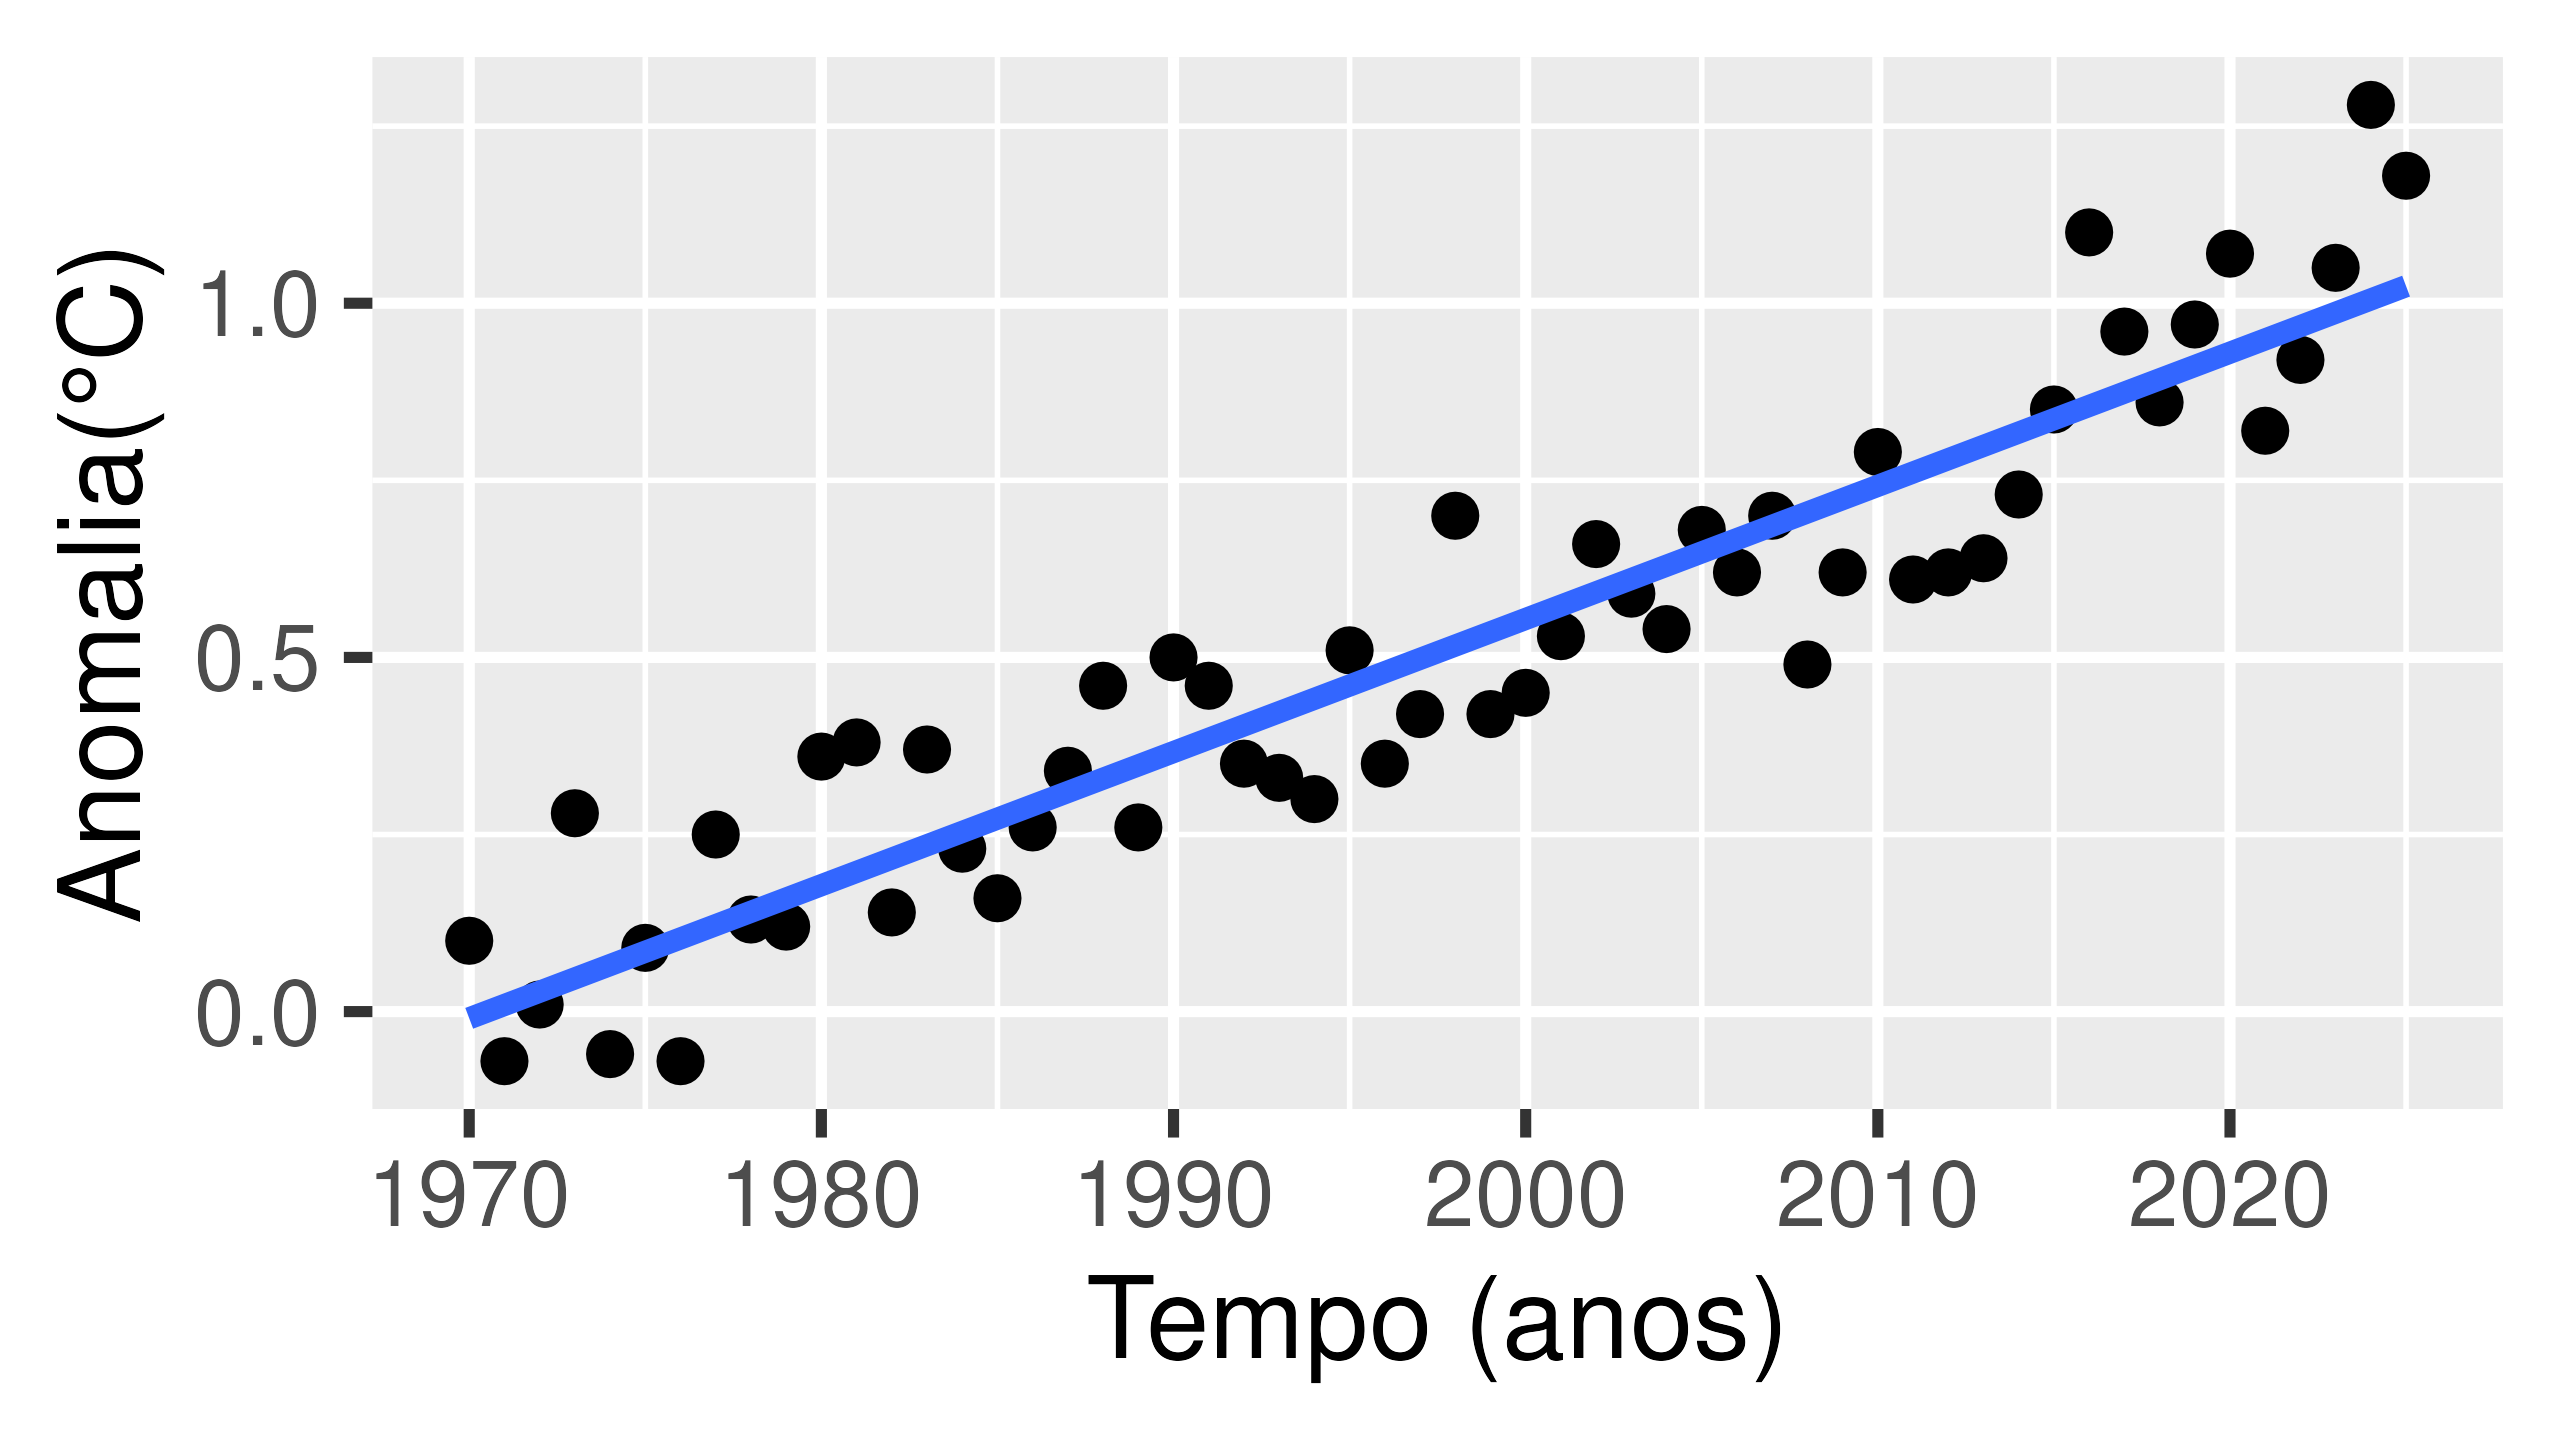
\includegraphics[width=\linewidth]{static/R/plot/anom-3-scatter+reg.png}
    \label{fig:2:anom-3-scatter+reg}
\end{figure}

Antes, foi dito que $\beta_1$ representava a inclinação da reta.
Além disso, ele cumpre uma outra função importante: representar a \textit{taxa de variação} da reta; como a unidade de medida em questão é anos, isso significa quanto a temperatura vai variar por ano.
A regressão realizada nesse conjunto de dados revela que a anomalia de temperatura média global cresce em um ritmo de $0,01879 °C$ ao ano.

Perceptivelmente, essa anomalia vem crescendo mais nos últimos anos do que vinha anteriormente, devido às mudanças climáticas.
O modelo de reta, por ter que simplificar drasticamente, é incapaz de expressar isso, de tal modo que nos últimos três anos sua estimativa está abaixo do valor real.
Geralmente, o que importa não é o quão próximo o modelo está dos dados já existentes, mas sim o quão bem o modelo se dá com extrapolar esses dados e, literalmente, prever o futuro.
Dadas essas tendências recentes, esse modelo pode não ser tão útil, uma vez que não detêm a habilidade de contemplá-las suficientemente.
Um modelo melhor, nesse caso, ao invés de uma reta usaria uma curva.
Por exemplo

\begin{figure}[H]
    \centering
    \caption{Gráfico da anomalia (°C) em função do tempo (anos), 1970-2025, com regressão linear e aproximação polinomial}
    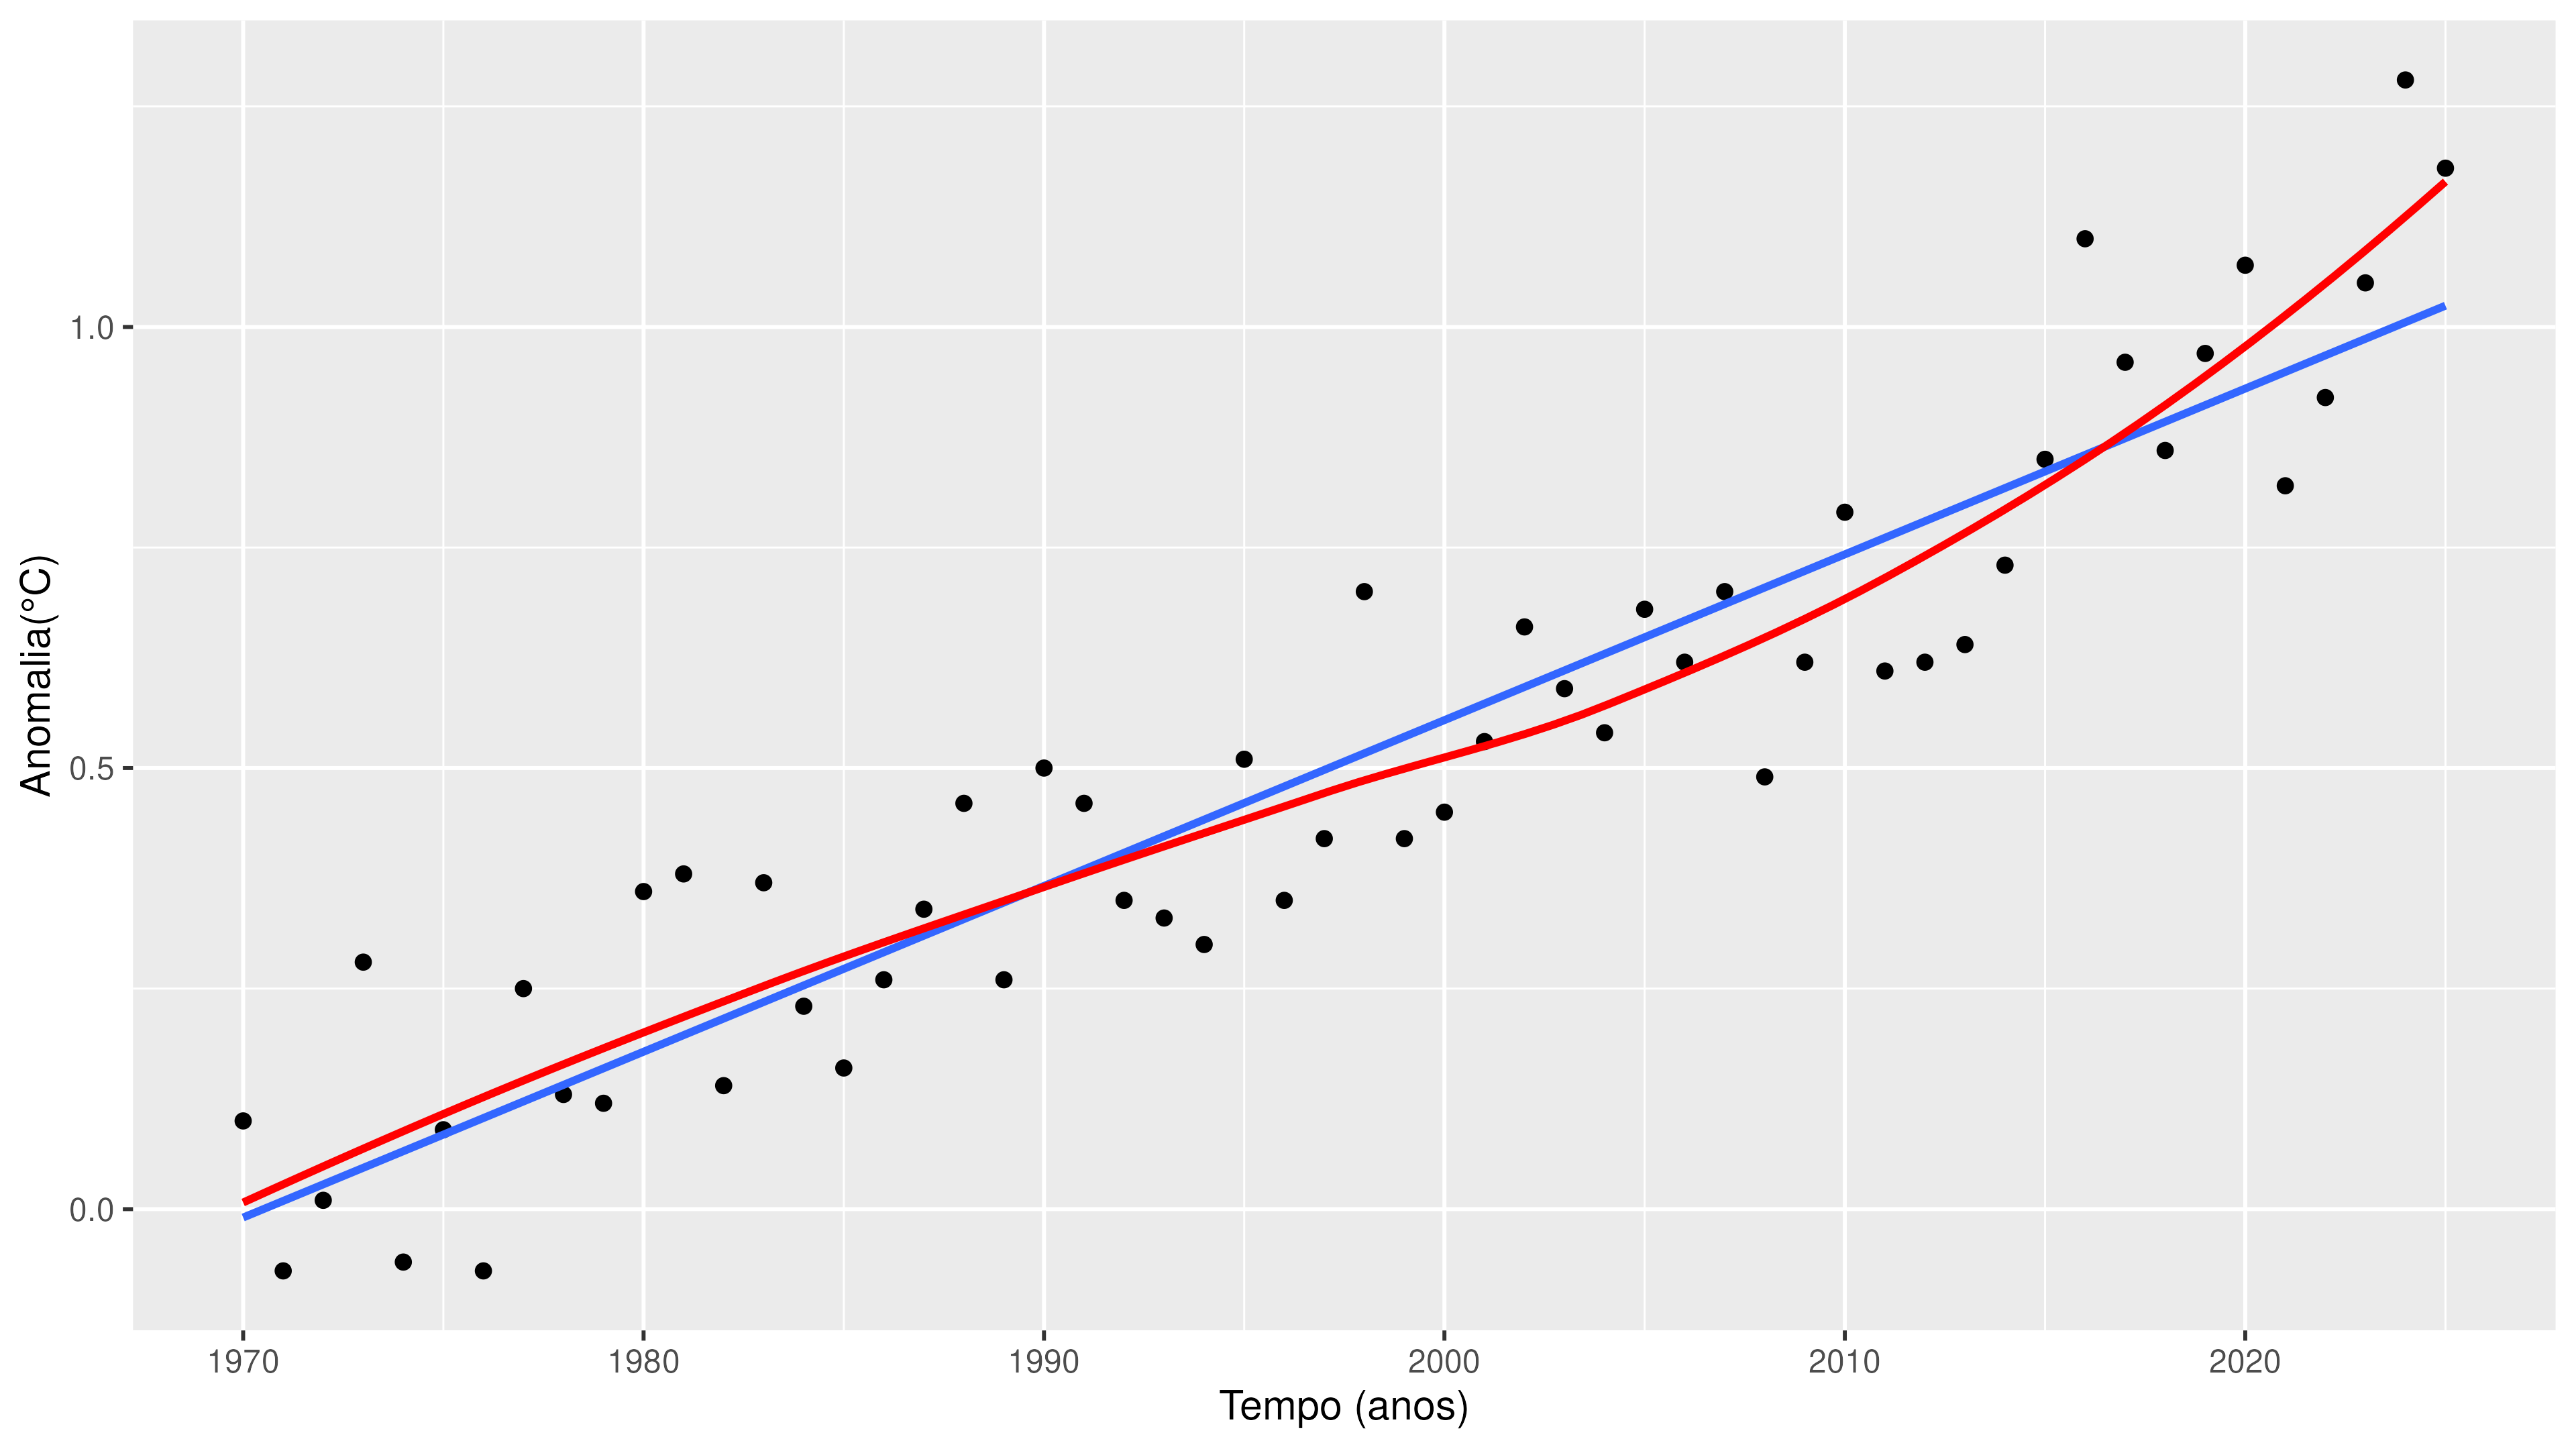
\includegraphics[width=\linewidth]{static/R/plot/anom-5-scatter+reg+poly.png}
    \label{fig:2:anom-3-scatter+reg+poly}
\end{figure}
